%%%%%%%%%%%%%%%%%%%%%%%%%%%%%%%%%%%%%%%%%%%%%%%%%%%%%%%%%%%%%%%%%%%%%%%%%%%

\documentclass{standalone}

\usepackage{amsmath}
\usepackage{mathptmx}
\usepackage{pgfplots}
\usetikzlibrary{external}
\tikzexternalize{cos-sin}
\pgfplotsset{compat=1.15}

%% IEEE uses Times Roman font, so we'll default to Times.
%% These three commands make up the entire times.sty package.
\renewcommand{\rmdefault}{ptm}
\renewcommand{\ttdefault}{pcr}
\normalfont\selectfont

\begin{document}

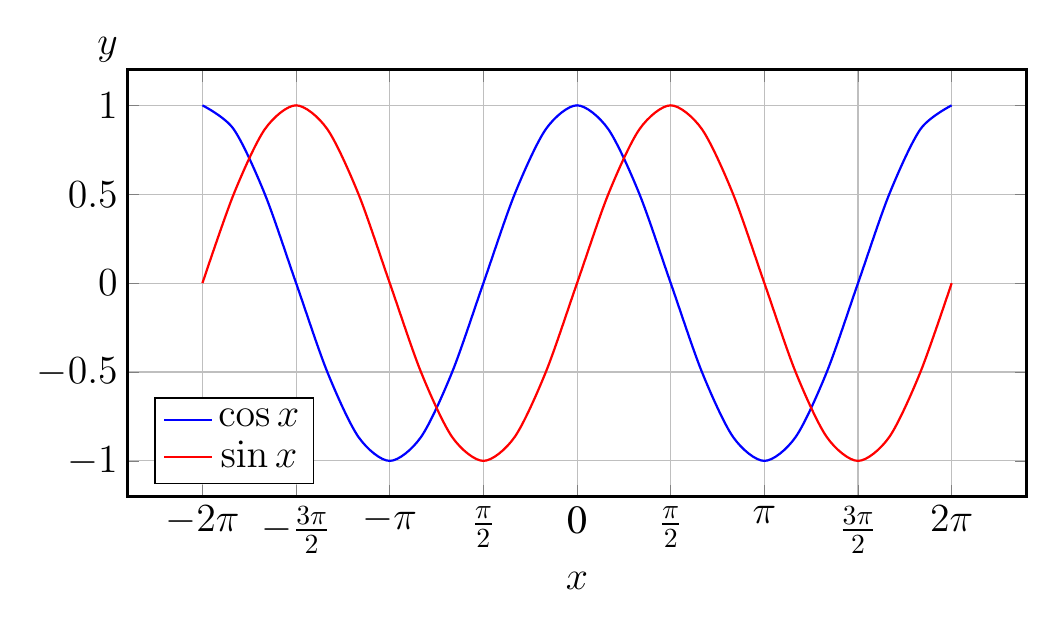
\begin{tikzpicture}
\tikzset{%%
  every mark/.append style={scale=1.0},%%
  scale=1.0%%
}
\pgfplotsset{%%
  every axis/.append style={font=\Large}%%
}

\begin{axis}[%%
  axis line style=very thick,%%
  enlargelimits=true,%%
  height=7cm,%%
  legend pos=south west,%%
  tick style={grid=major},%%
  trigStyle/.style={%%
    domain=-2*pi:2*pi,%%
    mark=none,%%
    smooth,%%
    thick%%
  },%%
  width=13cm,%%
  %%
  %% x-axis
  xlabel={\Large $x$},%%
  xtick={%%
    -6.283185,-4.712388,-3.141592,-1.570796,%%
    0,%%
    1.570796,3.141592,4.712388,6.283185%%
  },%%
  xticklabels={%%
    $-2\pi$,$-\frac{3\pi}{2}$,$-\pi$,$\frac{\pi}{2}$,%%
    0,%%
    $\frac{\pi}{2}$,$\pi$,$\frac{3\pi}{2}$,$2\pi$%%
  },%%
  %%
  %% y-axis
  every axis y label/.style={%%
    at={(axis description cs:0,1.1)},%%
    anchor=north east%%
  },%%
  ylabel={\Large $y$}%%
]
%%
%%
%% The function cos(x).
\addplot+ [trigStyle]
{cos(deg(x))};
\addlegendentry{$\cos x$}
%%
%%
%% The function sin(x).
\addplot+ [trigStyle]
{sin(deg(x))};
\addlegendentry{$\sin x$}
\end{axis}
\end{tikzpicture}

\end{document}
